\newpage

\section{Theorie}
\subsection{String \& StringBuffer}
Ein Objekt von String ist unveränderbar (immutable), d.h. es kann nach seiner Erstellung nicht mehr angepasst werden. Das macht es einfach um verschiedene Referenzen darauf zeigen zu lassen. Man muss sich keine Sorgen machen, dass eine Referenz das Original verändert. String bietet eigene Funktionen wie length, charAt, equals, equalsIgnoreCase, compareTo. \\ 
Merke: 'String + Irgendetwas (int, double etc)' ergibt einen neuen String und 'Irgendetwas + String' ergibt ebenfalls einen String. \\
Ein Objekt von StringBuffer kann mit den Funktionen, welche die Klasse StringBuffer bereitstellt einfach verändert werden (in der Länge und bezüglich des Inhalts). Die Buffer-Capacity bezeichnet die mögliche Buffergrösse, welche ohne Verlängerung möglich wäre. Die Buffer-Length gibt hingegen die aktuelle Anzahl enthaltener Zeichen an.  
\newline
\lstinputlisting{Loes/StringExample.java}
\lstinputlisting{Loes/StringPerformance.java}

\subsection{Ein- und Ausgabe}
Standard-Datenströme (engl. "standard streams")
sind vordefinierte Kommunikations-Kanäle zwischen
einem Computerprogramm und seiner Umgebung 
(Tastatur, Bildschirm). Die drei Standard-Datenströme \textbf{stdin (Standardeingabe), stdout (Standardausgabe) und stderr (Standardfehlerausgabe)} werden seit den 1970er Jahren praktisch von allen Betriebssystemen und Programmiersprachen unterstützt (Fortran bereits 1950) und für die Ein-/Ausgabe verwendet. Sie werden in der Regel bei allen Nicht-Gui-Programmen verwendet. Also bei Programmen, die in einem Terminalfenster ausgeführt werden und Eingabedaten von der Tastatur beziehen und Ausgabedaten in das Terminalfenster (Bildschirm) schreiben.Die drei Standarddatenströme können umgelenkt werden – das heisst, Eingabedaten aus einer Datei beziehen (statt von der Tastatur) oder Ausgabedaten in eine Datei schreiben (statt ins Terminalfenster). Das Programm merkt normalerweise nichts von einer solchen Umlenkung.

In Java werden die drei Standard-Datenströme durch folgende drei (statische) Objekte der Klasse System repräsentiert:
\begin{itemize}
	\item System.out repräsentiert die Standardausgabe – stdout .
	\\ Entspricht dem Terminalfenster bzw. der Console in Eclipse (wenn nicht umgelenkt). .println() wird darauf angewendet. Das heisst, dorthin (auf System.out) wird der Text "Hallo Welt" geschrieben. println() steht für "print line" das heisst, die Ausgabe wird automatisch durch einen Zeilenvorschub abgeschlossen. Möchte man keinen Zeilenvorschub am Ende, kann print() statt println()
	verwendet werden.\\
	Seit Java 5 gibt es zusätzlich zu println() und print() die Methode 
	printf(), welche analog der bekannten C-Funktion fprintf() mit einem 
	Formatstring arbeitet der Platzhalter beinhalten kann.s
	\item System.err repräsentiert die Standardfehlerausgabe – stderr.\\ Entspricht dem Terminalfenster bzw. der Console in Eclipse (wenn nicht umgelenkt).
	\item System.in repräsentiert die Standardeingabe – stdin. \\
	Sie entspricht der Tastatur (wenn nicht umgelenkt).
	Dabei werden die via Tastatur eingegebenen Zeichen vom Betriebssystem 
	zwischengespeichert. Erst nach der Eingabe von <Ret> (Betätigen der Return-Taste) wird das wartende 
	Java-Programm "aufgeweckt" und kann nun die Daten aus dem 
	Zwischenspeicher lesen und verarbeiten.
\end{itemize}

\lstinputlisting{Loes/EinlesenmitBufferRead.java}
\lstinputlisting{Loes/TextEinAusgabe.java} 
\lstinputlisting{Loes/EinlesenmitScanner.java}
\lstinputlisting{Loes/DemoScanner.java}

\subsection{Packages \& Import}
Packages sind Sammlungen von zusammengehörigen Klassen und bilden ein zusätzliches Strukturierungsmittel für Klassen. Pakete werden auf Datei-Verzeichnisse abgebildet, Klassen auf .java-Dateien. Eine \textbf{Compilation Unit} entspricht einer .java-Datei. Sie kann mehrere Klassendefinitionen enthalten, aber \textbf{nur eine public Klasse} (Klassenname / Dateiname). Ein Paket definiert den Namensraum und legt die Sichtbarkeit fest. Es kann aus mehreren Compilation Units bestehen. Pakete können zur Kapselung verwendet werden, da (nicht-public) Klassennamen nur im gleichen Paket sichtbar sind. Compilation Units (.java-Dateien) können nicht zur Kapselung verwendet werden, da sie keine Sichtbarkeitsgrenze aufweisen. \\
Regeln: \\
- Package-Anweisung muss erste Anweisung sein. \\
- Es ist höchstens eine Package-Anweisung pro Datei zulässig. \\
- Die .java-Datei muss sich in einer Verzeichnisstruktur befinden, 
welche dem Package-Namen entspricht. 
- Wenn die Package-Anweisung fehlt, gehören die Klassen zum 
sogenannten Default-Package. \\
-  Merke: Jede Klasse gehört zu einem Paket
\newline
\newline
\textbf{Wichtige Packages:}
\begin{itemize}
	\item java.lang System, String, Integer, Character, Object, Math, ...
	\item java.io File, InputStream, OutputStream, Reader, Writer, ...
	\item java.util Vector, Stack, ArrayList, BitSet, HashTable, Random, ...
	\item java.awt Button, CheckBox, Frame, Color, ... 
\end{itemize}
Eine import-Anweisung dient dazu die Namen von Klassen aus einem Package zu importieren. Danach können die Klassennamen direkt, d.h. ohne Package-Namen verwendet werden. \\
\lstinputlisting{Loes/import.java}

\subsection{Klassen}

Bei Java gibt es keine Trennung zwischen Deklaration und Definition (Header, C-File). Die Implementierung ist immer innerhalb einer Klasse. Zudem gibt es keine Initialisierungslisten. Die Übergabe von Parametern erfolgt immer by value. Bei Referenzen erfolgt eine "shallow copy" und keine "deep Copy". 
 Alle Attribute haben einen definierten Startwert (falls keiner gegeben - Initialisierung mit null oder 0.00). \\
 Ein Objekt ist eine Variable deren Datentyp durch eine Klasse (Referenzdatentypen) definiert ist.  
\begin{itemize}
	\item abstract: Von dieser Klasse kann kein Objekt instanziert werden. Nur diese Klassen können abstrakte Methoden enthalten. Dabei handelt es sich um Methoden, welche keine Implementierung besitzen. 
	\item final: Von dieser Klasse kann nicht weiter abgeleitet werden.
	\item public: Klasse ist öffentlich und überall verwendbar
	\item ohne public: Klasse ist nur im gleichen Paket verwendbar
	\item protect: Methoden und Attribute sind von Unterklassen und anderen Klassen im gleichen Package verwendbar
	\item finalize(): hat in Java praktisch keine Bedeutung und sollte vermieden werden. Sie entsprechen \textbf{nicht} den Destruktoren von C++. 
	\item static: \\
	- Statische Klassenmethoden: Ihr Aufruf erfolgt mit dem Klassennamen. Sie ersetzen die globalen, freien Funktionen, aus C++ welches es in Java nicht gibt (z.B. java.lang.Math).  \\
	Bsp: double z = Math.sqrt(x); \\
	- Statische Klassenattribute: Zugriff erfolgt über den Klassennamen. Sie existieren genau ein Mal in der Klasse und werden oft zur Definition von Konstanten verwendet. \\
	Bsp: final static int SIZE = 100; \\
	- Statischer Block: Dieser Teil wird ausgeführt, wenn die Klasse geladen wird (static initializer). \\
	Bsp.: class Ufo \{ static \{ */ Initialisierung */  \}\} \\
	- import static java.xx.bbb.*/yy : Importiert alle (oder nur eine) statische Methoden und Attributen der Klasse bbb. Nun können alle statischen Methoden und Attribute direkt - also ohne Klassenname verwendet werden. \\
	Bsp.: import static java.lang.Math.*; \\
	double z = PI * sqrt( sin(x) + cos(y));
	\item synchronized: Methode kann nicht unterbrochen werden
	\item final: Bezeichnen Konstanten und werden damit "read only"
\end{itemize}

\subsubsection{Vergleiche}
Vergleiche mit == und != beziehen sich auf die Referenzen also die Adressen und nicht auf den Inhalt des Referenzobjekts. \\ 
Person p1= new Person("Meier"); \\
Person p2= new Person("Meier"); \\
if (p1 == p2) System.out.println("gleich"); \\
else  System.out.println("ungleich"); \\
Ausgabe: ungleich, denn die Adresse von p1 und p2 sind nicht dieselben. \\
Vergleiche mit .equals() erfolgt ein inhaltlicher Vergleich.
if(p1.equals(p2)) wäre besser. Für eigene Klassen muss die Methode equals() überschrieben werden. \\
Die Methode int hashCode() aus der java.lang.Object-Bibilothek kann ebenfalls für Vergleich verwendet werden. Dabei wird ein int-Wert aus den Attributen des Objektes berechnet. Damit kann effizient bestimmt werden, ob 2 Objekte sicher verschieden sind, denn dann sind die Hash-Codes ungleich. Es kann jedoch nicht mit Sicherheit bestimmt werden, ob die Objekte gleich sind. Das muss dann noch mit equals geprüft werden. Achtung: Immer wenn equals überschrieben wird, ist auch die Funktion hashCode() zu überschreiben!\\
\subsection{Vererbung}
In Java gibt es keine Mehrfachvererbung bei Klassen. Es kann nur von einer Klasse geerbt (A extends B) werden, aber eine Klasse kann mehrere Interfaces (A implements C, D, E) haben. Die abgeleitete Klasse erweitert die Basisklasse. Es wird zuerst der Konstruktor der Basisklasse aufgerufen (falls keiner vorhanden wird eine Default-Konstruktor erzeugt) und dann jener der abgeleiteten Klasse. Dem Konstruktor der Basisklasse kann mit super (xxx) auch ein Parameter übergeben werden. Die abgeleitete Klasse erbt die Methoden der Basisklasse, kann diese überschreiben und auch neue Methoden hinzufügen. Konstruktoren haben keine Initialisierungslisten. 
\begin{itemize}
	\item this: ist vom Typ des aktuellen Objektes und kann verwendet werden, wenn der übergebene Parameter gleich heisst, wie das Attribut der Klasse.  \\
	Bsp.: public class Person \{ //
	private string name; //
	public Person(String name) //
	\{	this. name = name \} \} //
	\item super: ist vom Typ der unmittelbar darüberliegenden Oberklasse	\\
	super.super ist illegal
\end{itemize}  
Eine Referenz von einer Oberklasse darf auf eine Objekt einer davon abgeleiteten Klasse zeigen. Beim Aufruf der Methode wird in Java gemäss dem "late Binding" die Klasse der referenzierten Klasse verwendet. \\
Bsp.: Person person = new Student("Meier", 1298); \\
pers. print();  // Das print() der Klasse Student wird aufgerufen.
\newline
\newline
\textbf{Up- und Downcasting: } Ein Objekt einer abgeleiteten Klasse Sparkonto kann an ein Objekt der Oberklasse Konto übergeben werden. Ob eine Oberklasse an ein Objekt der abgeleiteten Klasse übergeben bzw. dazu umgewandelt werden kann, muss mit \textbf{instanceof} zuerst geprüft werden. 

\lstinputlisting{Loes/Downcasting.java} 
\textbf{Instance Initializer: } Code-Block, der nach dem Konstruktor der Oberklasse und vor dem Konstruktor der Klasse bei der Erzeugung eines Objekts aufgerufen wird. Sie werden bei anonymen Klassen verwendet, welche keine Konstruktoren haben.  
\lstinputlisting{Loes/Initializer.java}
\subsubsection{Klassenverschachtelung}

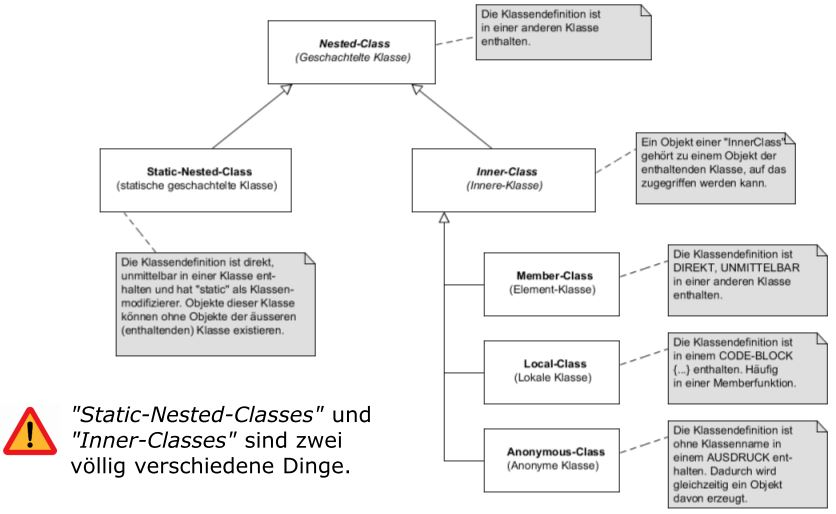
\includegraphics[width=0.50\textwidth]{Loes/NestedClass.jpg}

Die \textbf{Element-Klasse} wird innerhalb der äusseren Klasse aber nicht innerhalb des Konstruktors definiert. \\ 
Die \textbf{lokale Klasse} wird innerhalb des Konstruktors definiert. \\
\textbf{Anonyme Klasse} wird innerhalb eines Funktionsaufrufs innerhalb des Konstruktors definiert. \\

\subsection{Interfaces}
Ein Java-Interface ist eine Menge von Methodendeklarationen ohne Implementierung (\textbf{abstract}) und konstanten Werten. Dabei sind alle Methoden automatisch public und abstract und alle Werte public und static final.
\lstinputlisting{Loes/Interface.java}
Eine Klasse kann ein Interface implementieren (\textbf{implements}) und erbt dadurch alle Methoden. Da diese jedoch abstract sind, muss sie \textbf{alle, ausser die Default} Methoden überschreiben und implementieren. Referenzen von Interfaces können wie abstrakte Klassen verwendet werden. Eine Klasse kann mehrere Interfaces implementieren.\\
Interfaces können von anderen Interfaces erben mit \textbf{extends} und das ganze wird Schnittstellenvererbung genannt. \\

\textbf{Änderungen bei Interfaces ab Java 8}\\
- Default-Methoden bei Interfaces dienen zur Erweiterung von bestehenden Interfaces, ohne dass die Klassen, welche bereits diese Interfaces implementieren geändert werden müssen. Die default-Implementierung wird dann verwendet, wenn eine Klasse die entsprechende Methode des Interfaces nicht selbst implementiert. \\
- Statische Interface Methoden zusätzliche Methoden innerhalb eines Interfaces, welche aber in den Klassen die diese Interfaces implementieren, nicht überschrieben werden können.\\
- Funktionale Interfaces (nur neuer Begriff) sind Interfaces welche genau eine abstrakte Methode enthalten. Sie sind wichtig im Zusammenhang mit sogenannten Lambda-Ausdrücken. Das Package java.util.functions enthält 40 funktionale Interfaces. In der Praxis werden neu dort Lambda-Ausdrücke eingesetzt, wo früher i.a.R. anonyme Klassen verwendet wurden.  
\lstinputlisting{Loes/Interface2.java}

\subsection{Lambdas}
Lambda-Ausdrücke ermögliche eine besonders kompakte Implementierung von funktionalen Schnittstellen (Interfaces), d.h. Interfaces mit genau einer abstrakten Methode. Dies werden häufig anstelle von  anonymen Klassen verwenden. Sie erlauben ebenfalls einen direkten Zugriff auf die Variablen der Umgebung (!).

\lstinputlisting{Loes/Lambda.java}

Sowohl mit einem Lambda-Ausdruck als auch einer anonymen Klasse kann auf kann auf die Umgebung zugegriffen werden. Der Code mit dem Lambda-Ausdruck ist jedoch kompakter und übersichtlicher. Man muss da aber das zugrunde liegende Interface kennen. Ein Lambda-Ausdruck ist daran erkennbar, dass er einen Pfeil-Operator 
enthält. Innerhalb eines Lambda-Ausdrucks kann .super und .this verwendet werden. 
\newline
\newline
Ein Lambda-Ausdruck besteht aus::\\
- Interface-Namen (optional): Name des zugrunde liegenden 
Interfaces, eingeschlossen in runden Klammer.\\
- Parameterliste: Liste von durch Komma getrennten formalen 
Parametern, eingeschlossen in runden Klammern. Die Datentypen bei den Parametern können dabei weggelassen werden. \\
- Pfeil-Operators  $\rightarrow$ \\
- Body: aus einem einzelnen Ausdruck (ohne ";") oder aus einem Anweisungsblock, das heisst, mehrere Anweisungen eingeschlossen in "{    }".

\subsection{Exception Handling}
Beim Exception Handling in Java wird beim Auftreten eines Fehlers im geschützten Block die Ausführung dessen abgebrochen, der Fehlerbehandlungscode ausgeführt und dann der geschützt Block weitergeführt (wie Interupts). Dadurch kann der fehlerfreie Fall von den Fehlerfällen sauber getrennt werden. Zudem kann man keinen Fehler vergessen, da der Compiler prüft, ob zu jeder möglichen Ausnahme ein Behandlung existiert. Achtung: Die speziellen Exception-Typen müssen vor den allgemeienn Exception-Typen liegen. Am Ende wird oftmals ein finally eingefügt, damit gewisse Abschlussarbeiten wie z.B. das Schliessen eines Dokuments auch im Fehlerfall ausgeführt wird.\\

\lstinputlisting{Loes/Exceptions.java}

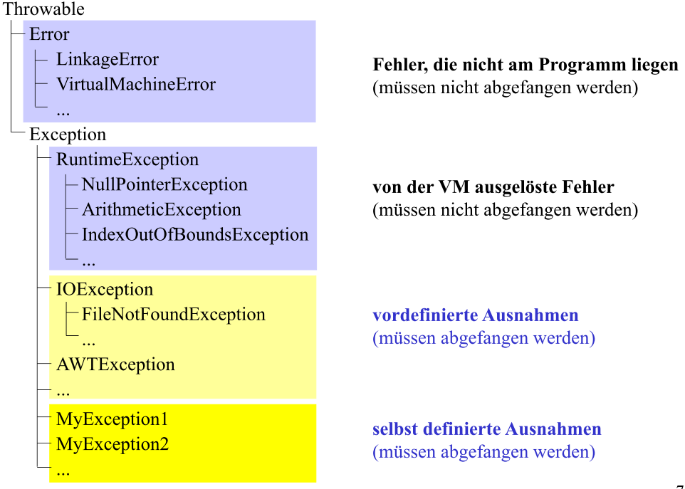
\includegraphics[width=0.40\textwidth]{Loes/Exceptions.png}
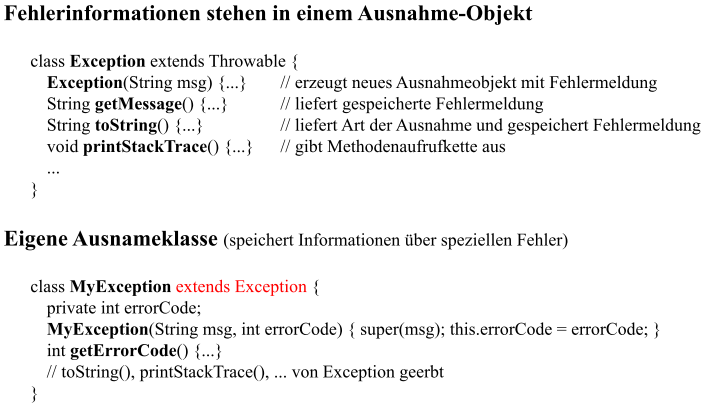
\includegraphics[width=0.50\textwidth]{Loes/Exceptions3.png}

public static void main(String[] args) \textbf{throws Exception} wird im Funktionskopf angegeben, wenn auf die Standard Exceptions der in der Funktion enthaltenen Methoden zurückgegriffen werden. Das heisst, dass nicht alle Exceptions im Programm selbst behandelt werden sollen ("Quick and Dirty Programming). 

 
                      
\subsection{GUI}
\subsubsection{AWT - Abstract Window Toolkit}
AWT verwendet die GUIs des zugrundeliegenden Betriebssystems. Deshalb sind die Plattform-Eigenheiten  nicht völlig eliminierbar. Es hat eine beschränkte Funktionalität, da es dem kleinsten gemeinsamen Nenner der verschiedenen Plattformen entspricht. 

\subsubsection{Swing}
Die GUI-Elemente werden in Java "erstellt". Dadurch ist das "Look and Feel" anpassbar (standardmössig L\&F des Betriebssystems). Es kann zur Laufzeit umgeschaltete werden. Zudem ist der Funktionsumfang sehr gross. Es baut auf Teilen von AWT auf, ersetzt jedoch auch gewisse Teile. Intern wird die MVC-Architektur verwendet. 

\subsubsection{Event Handling}
Ein Framework ist ein Programmgerüst, in das vom Programmierer das Anwendungsprogramm eingebettet wird. Aus dem Framework heraus werden Funktionen des Anwendungsprogramms aufgerufen (Hollywood-Prinzip). 
Je nach Ereignisart werden verschiedene Event-Typen unterscchieden. Diese werden unterteilt in High-Level-Events, Intermediate-
Level-Events und Low-Level-Events. \\
\newline
\textbf{Varianten zur Implementierung des Event Handlings} 
\textbf{Variante 1: Listener in der Hauptklasse} \\
die Hauptklasse implementiert das Listener-Interface. \\
z.B. public class MyFrame extends JFrame implements ActionListener \\
Nachteil: es gibt nur einen Listener auch bei mehreren Buttons. \\
\textbf{Variante 2: Listener als externe Klassen} \\
für jeden benötigten Listener wird eine eigene Klasse erstellt.\\
z.B.  IncButtonListener implements ActionListener { ... }  \\
DecButtonListener implements ActionListener { ... } \\
Nachteil: zusätzliche Klassen, welche eine Konstruktor benötigen. \\
\textbf{Variante 3: Listener als innere (anonyme) Klassen} \\
Bsp:  decButton.addActionListener (new ActionListener() {  ...  });\\
Vorteile:    Zugriff zur Hauptklasse möglich, pro Button eigener  Listener.  \\
Nachteil:  etwas unübersichtlich. \\
\textbf{Variante 4: Listener als Lambda-Ausdrücke (seit Java 8)} \\
Für jeden benötigten Listener wird ein Lamda-Ausdruck erstellt. Dabei kann der Funktionskopf ("void actionPerformed(ActionEvent e)" weggelassen werden.\\
Bsp:   event -> label.setText("Anz = " + --anzahl) \\
Vorteile: Zugriff zur Hauptklasse möglich, pro Button eigener Listener, kompakt.
\newline
,\newline
\subsubsection{Layout Manager}

Beim \textbf{GridLayout} wird die Anzahl Zeilen und Spalten im Konstruktor angeben. Die Reihenfolge von add() bestimmt die Anordnung. Bei einem 2-dimensionalen Grid gehts zuerst hinuntern und dann nach rechts. Alle Zellen gleich gross.\\
Beim \textbf{FlowLayout} sind die Zellen so breit wie der Text darin. \\
Beim \textbf{BorderLayout} müssen nicht alle Zellen gleich gross sein. Die Zelle im Zentrum wird maximiert und jene an den Rändern minimiert. Bei add() muss eine Position mit den Himmelsrichtungen angegeben werden. \\
Beim \textbf{CardLayout} werden verschiedene Layout kombiniert. \\

\subsection{AWT- \& Swing Komponenten}
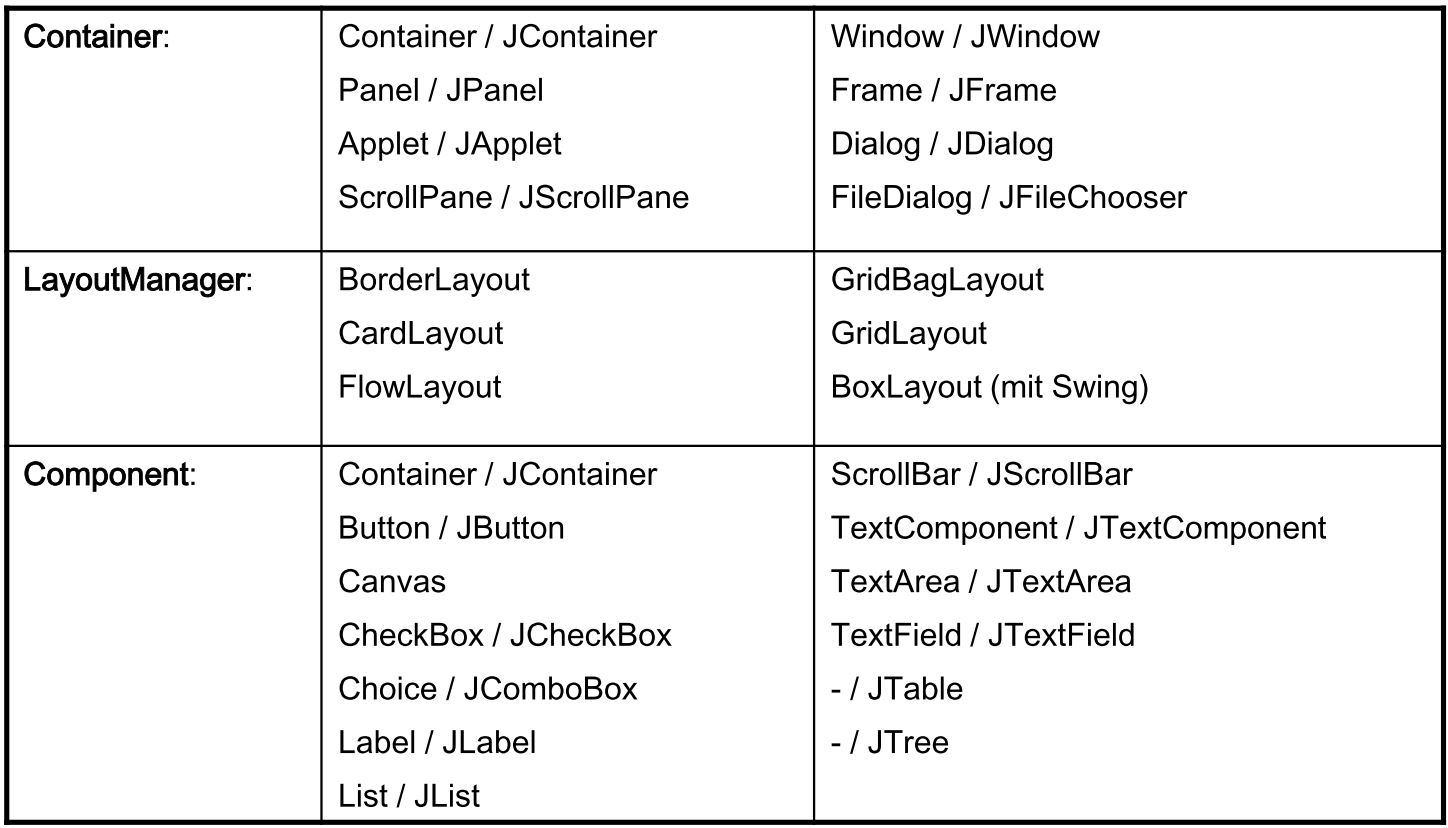
\includegraphics[width=0.50\textwidth]{Loes/Komponenten.JPG}

\subsection{Others}
Bezüglich Binding entsprechen die abstrakten Klassen von Java den virtuellen Klassen von C++. \\
Der Garbage Collector kann explizit mit dem Befehl \textbf{ja
	va.lang.System.gc() }  resp.  \textbf{java.lang.Runtime.gc()} aufgerufen werden. \\
Arrays werden wie alle Objekte bei Java auf dem Heap mit new erzeugt und als Referenz zurückgegeben. Deshalb gehören sie im Gegensatz zu C++ zu den Referenzdatentypen. \\

\textbf{Java vs. C++} \\
(+) Java hat ein integriertes Speichermanagement mit dem Garbage Collector, was bei C++ selbst gemacht werden muss.  \\
(+) Java ist plattformunabhängig.  \\
(+) Java verfügt über umfassende Klassenbibliotheken (auch für die GUI Programmierung). \\
(--) Java kann einfacher Reverse Engineered werden. \\
(--) C++ ist schneller. \\
(--) Für die Verwendung von Java benötigt man eine Java Virtual Machine mit einer JRE (Java Runtime Environment) auf dem ausführenden Gerät. 

\section{Papierübungen}
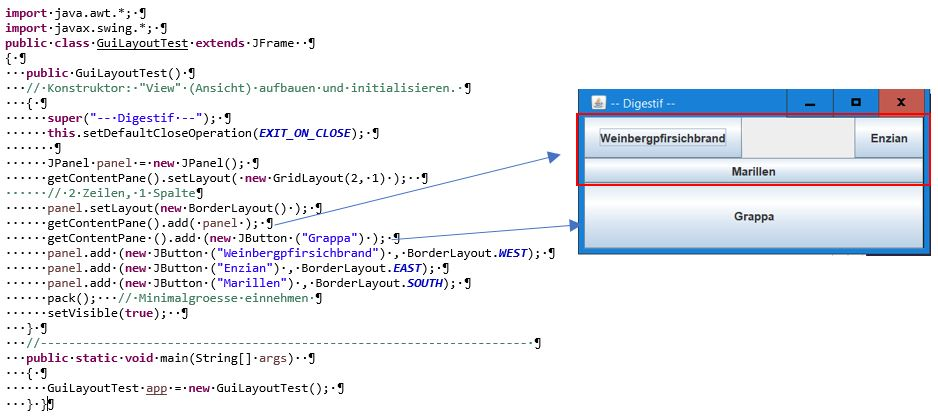
\includegraphics[width=0.99\textwidth]{Loes/Papieruebung.JPG}
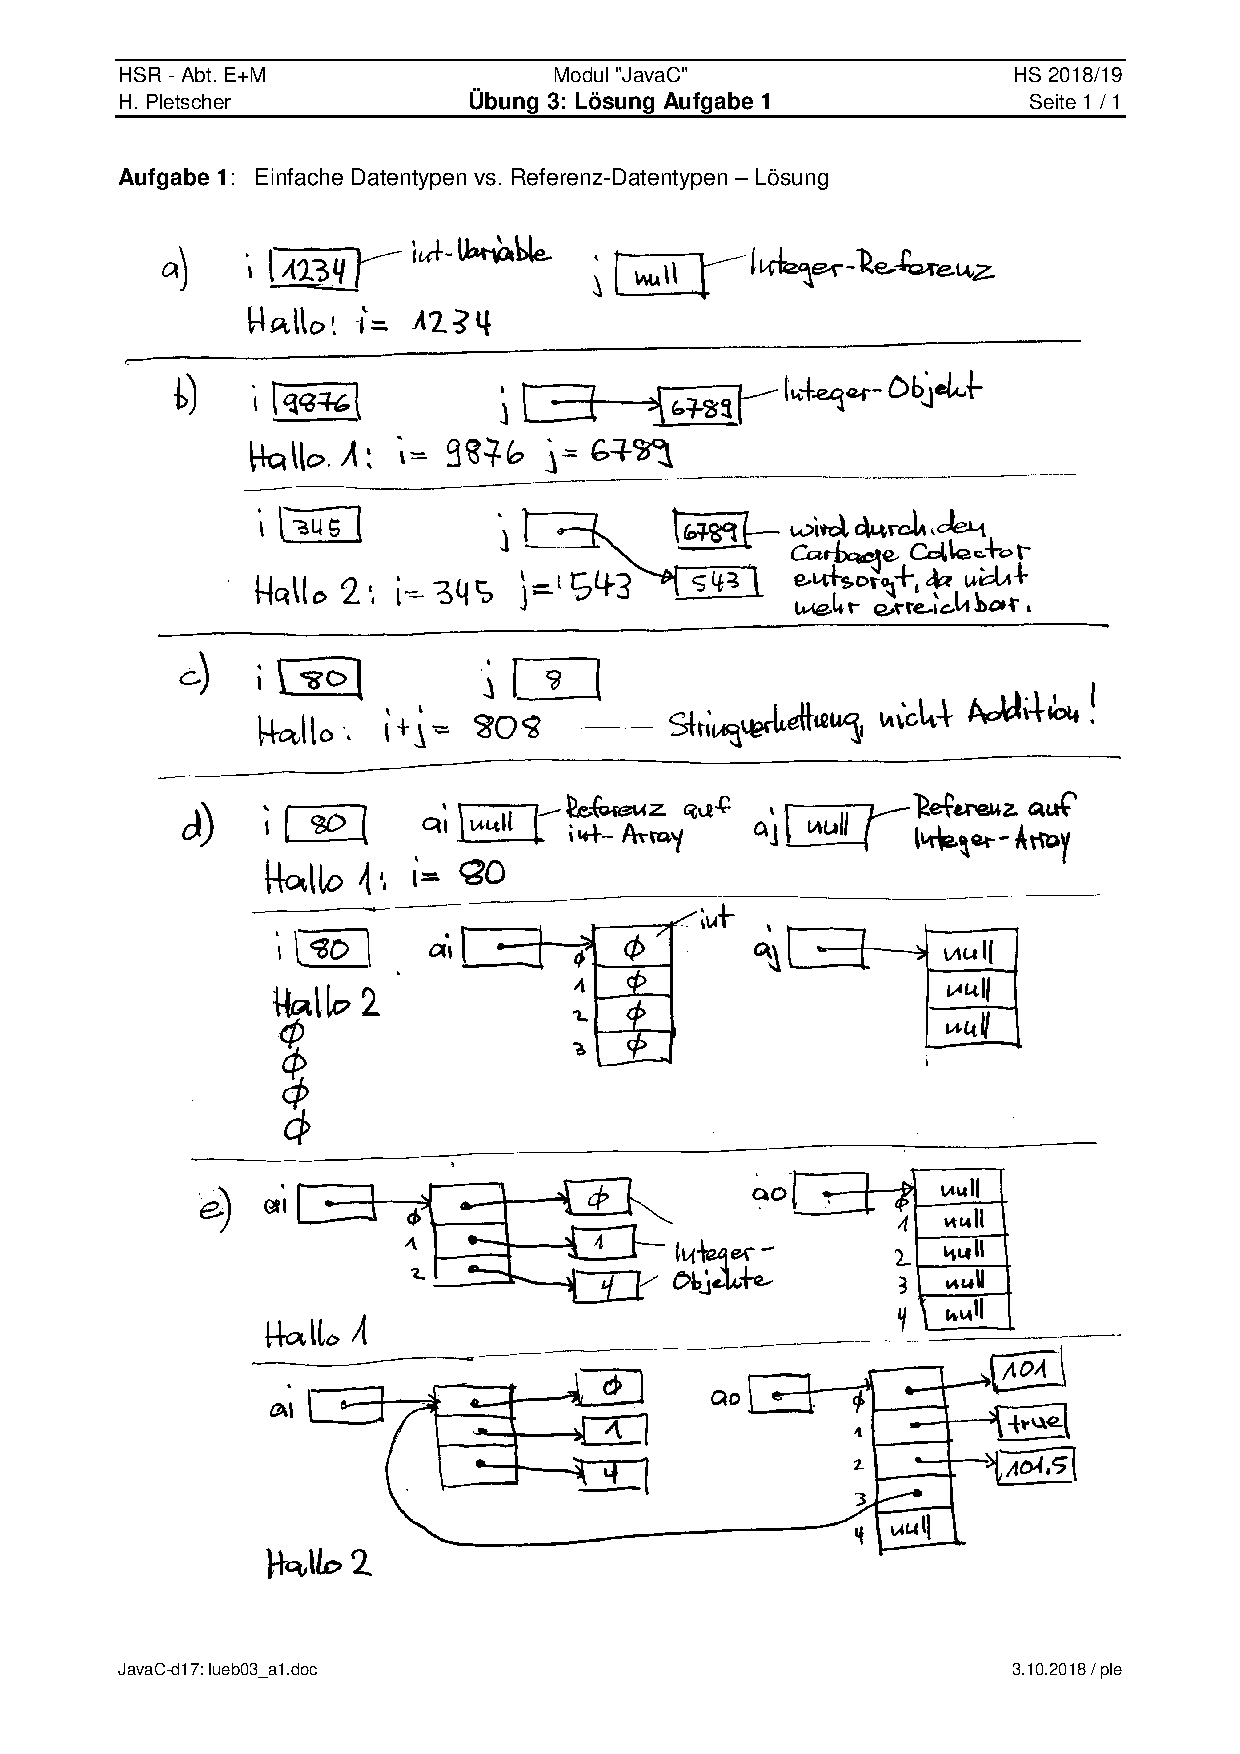
\includepdf[scale=0.9]{Loes/lueb03A1.pdf}
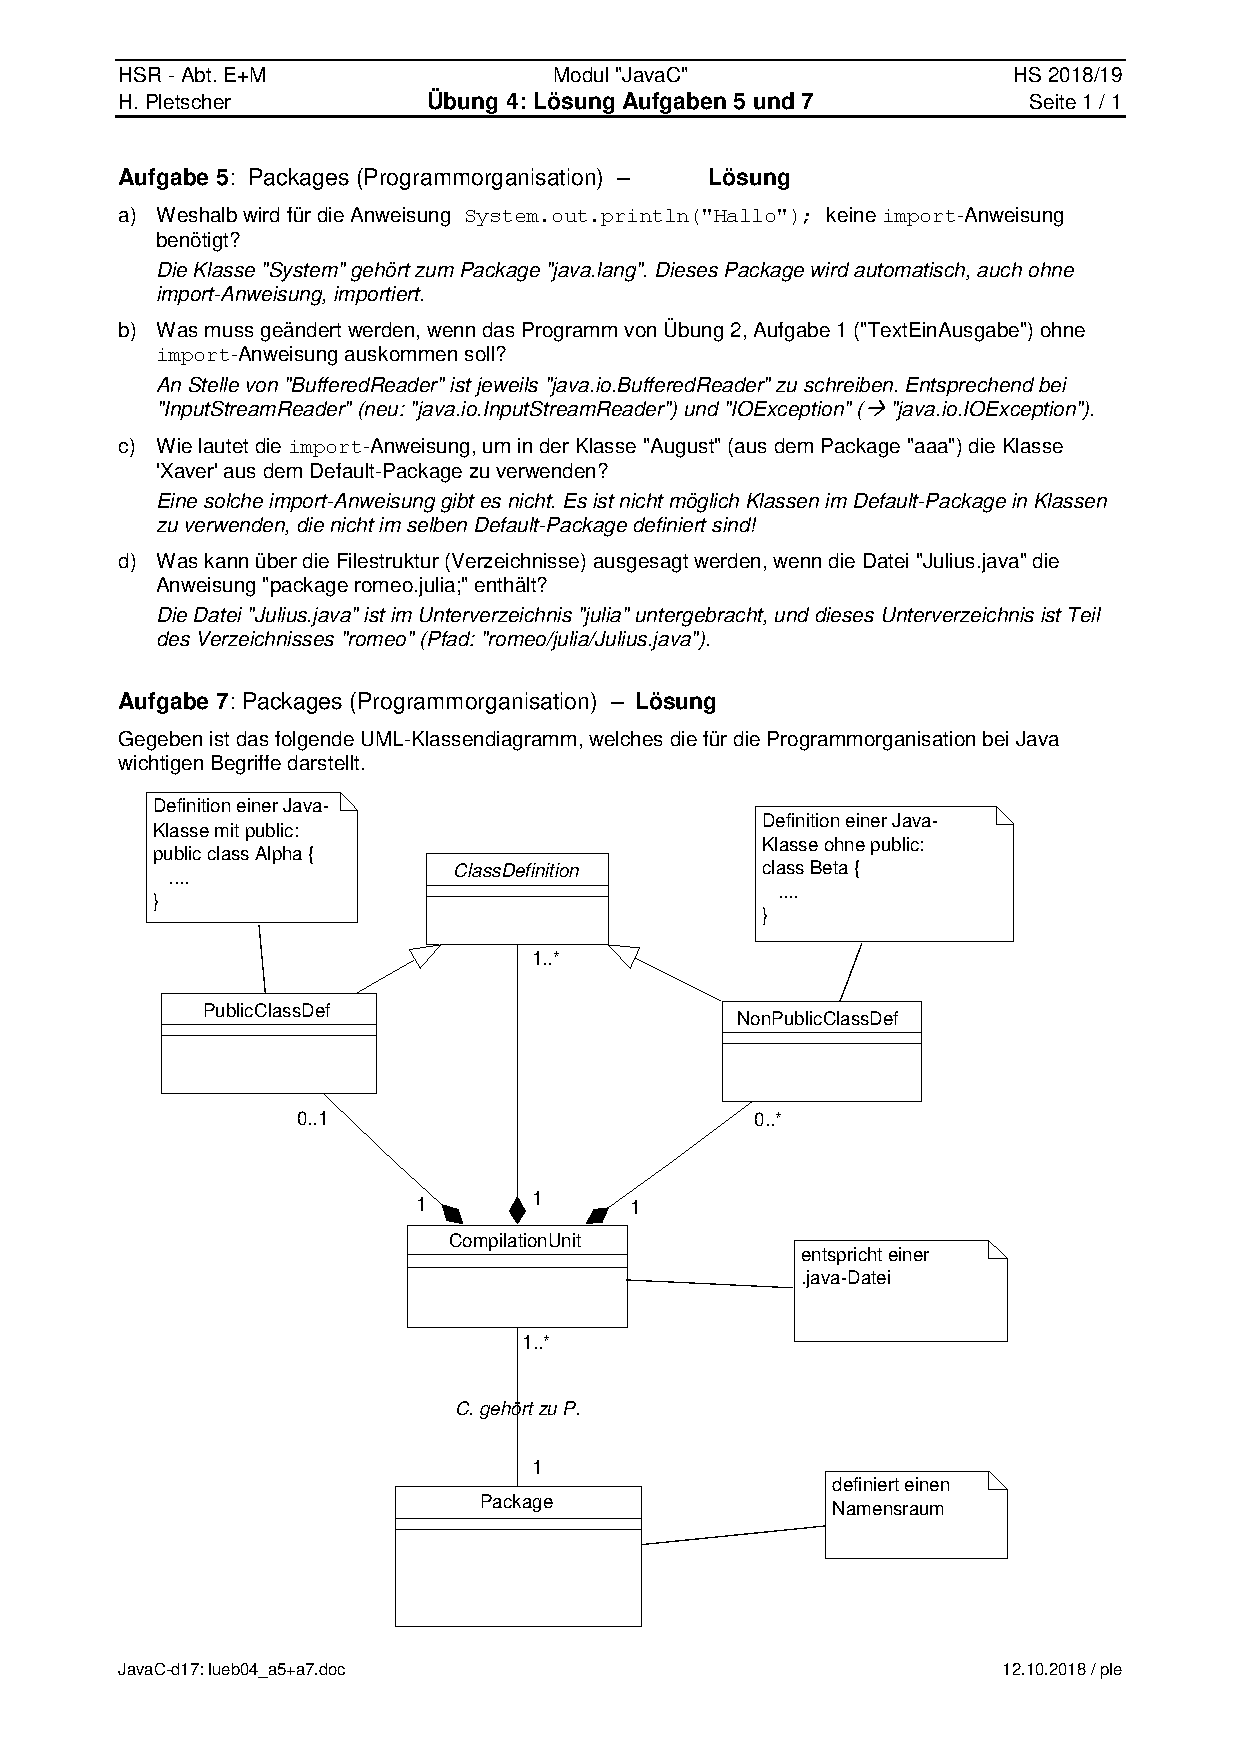
\includepdf[scale=0.9]{Loes/lueb04A5A7.pdf}
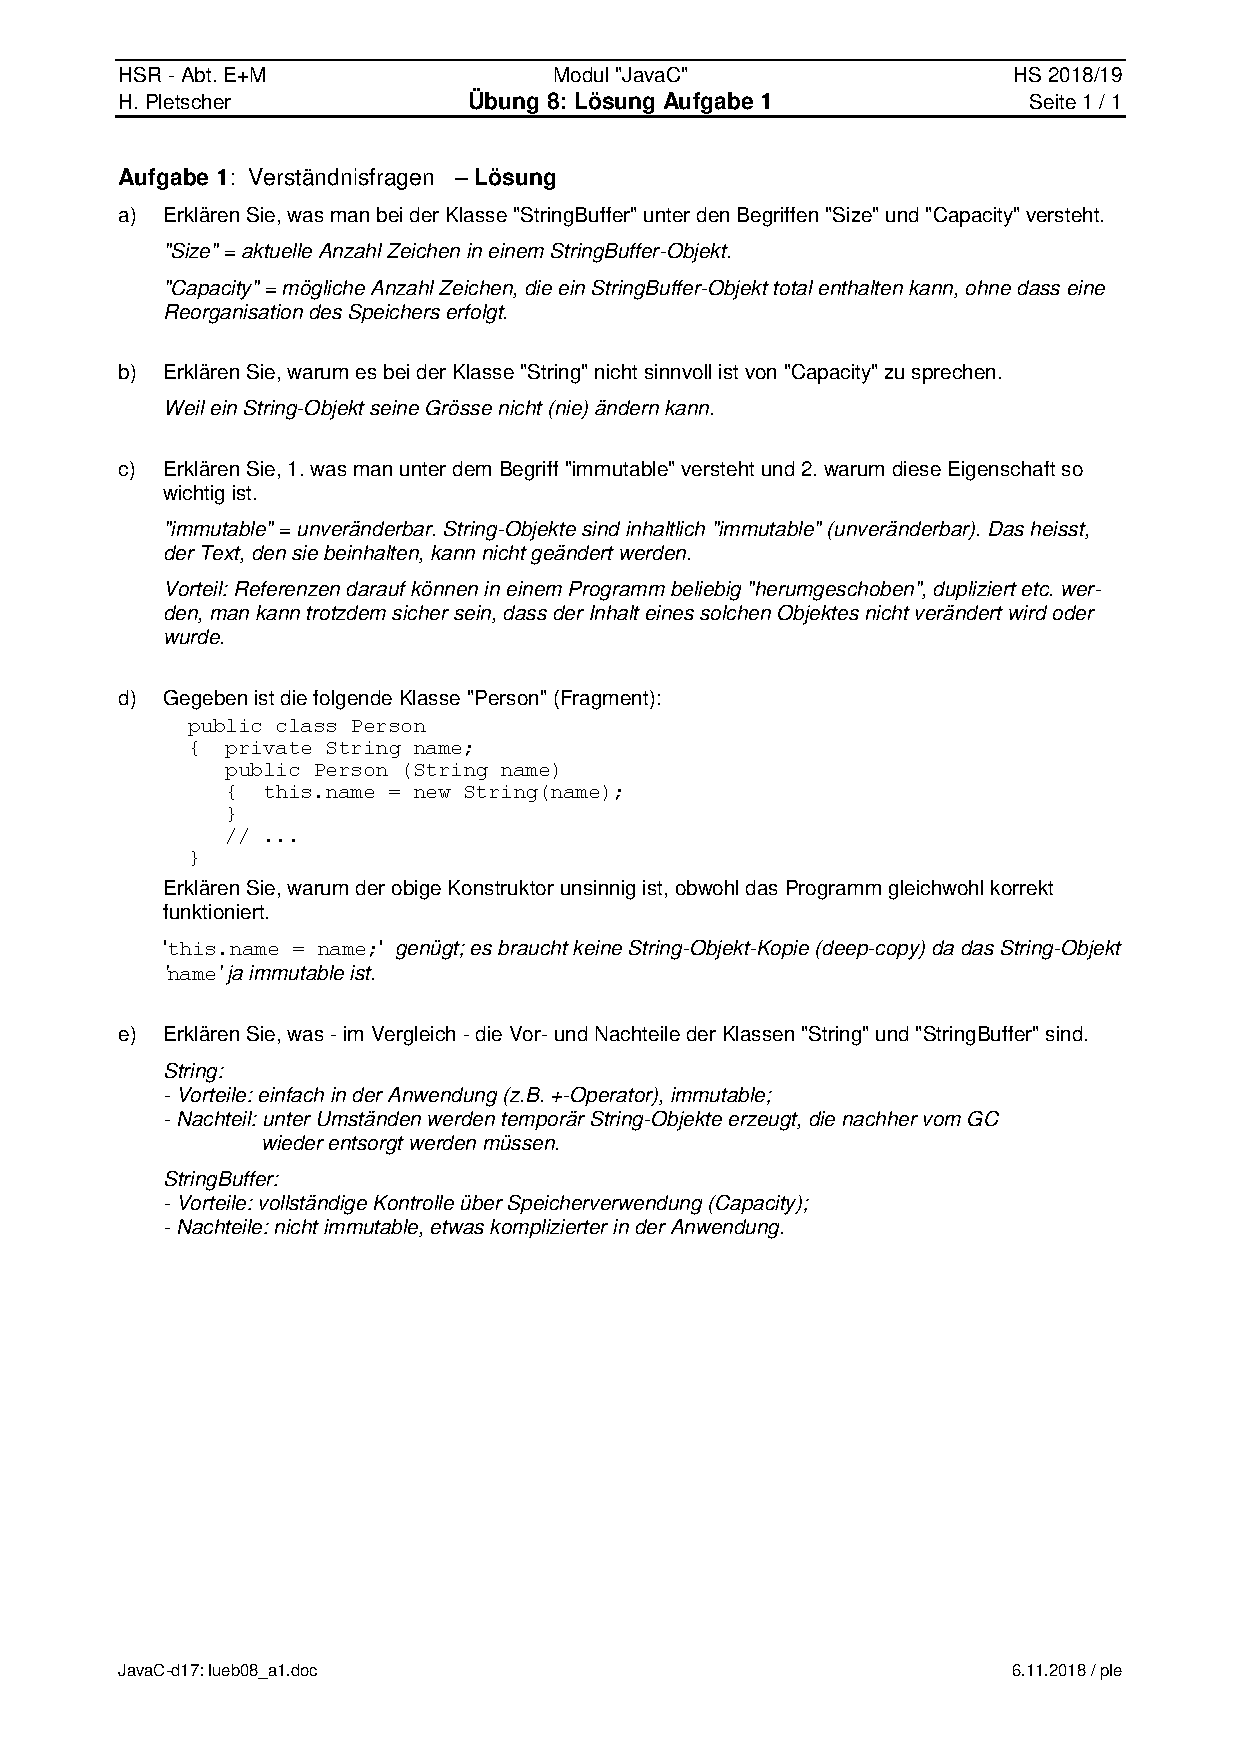
\includepdf[scale=0.9]{Loes/lueb08A1.pdf}
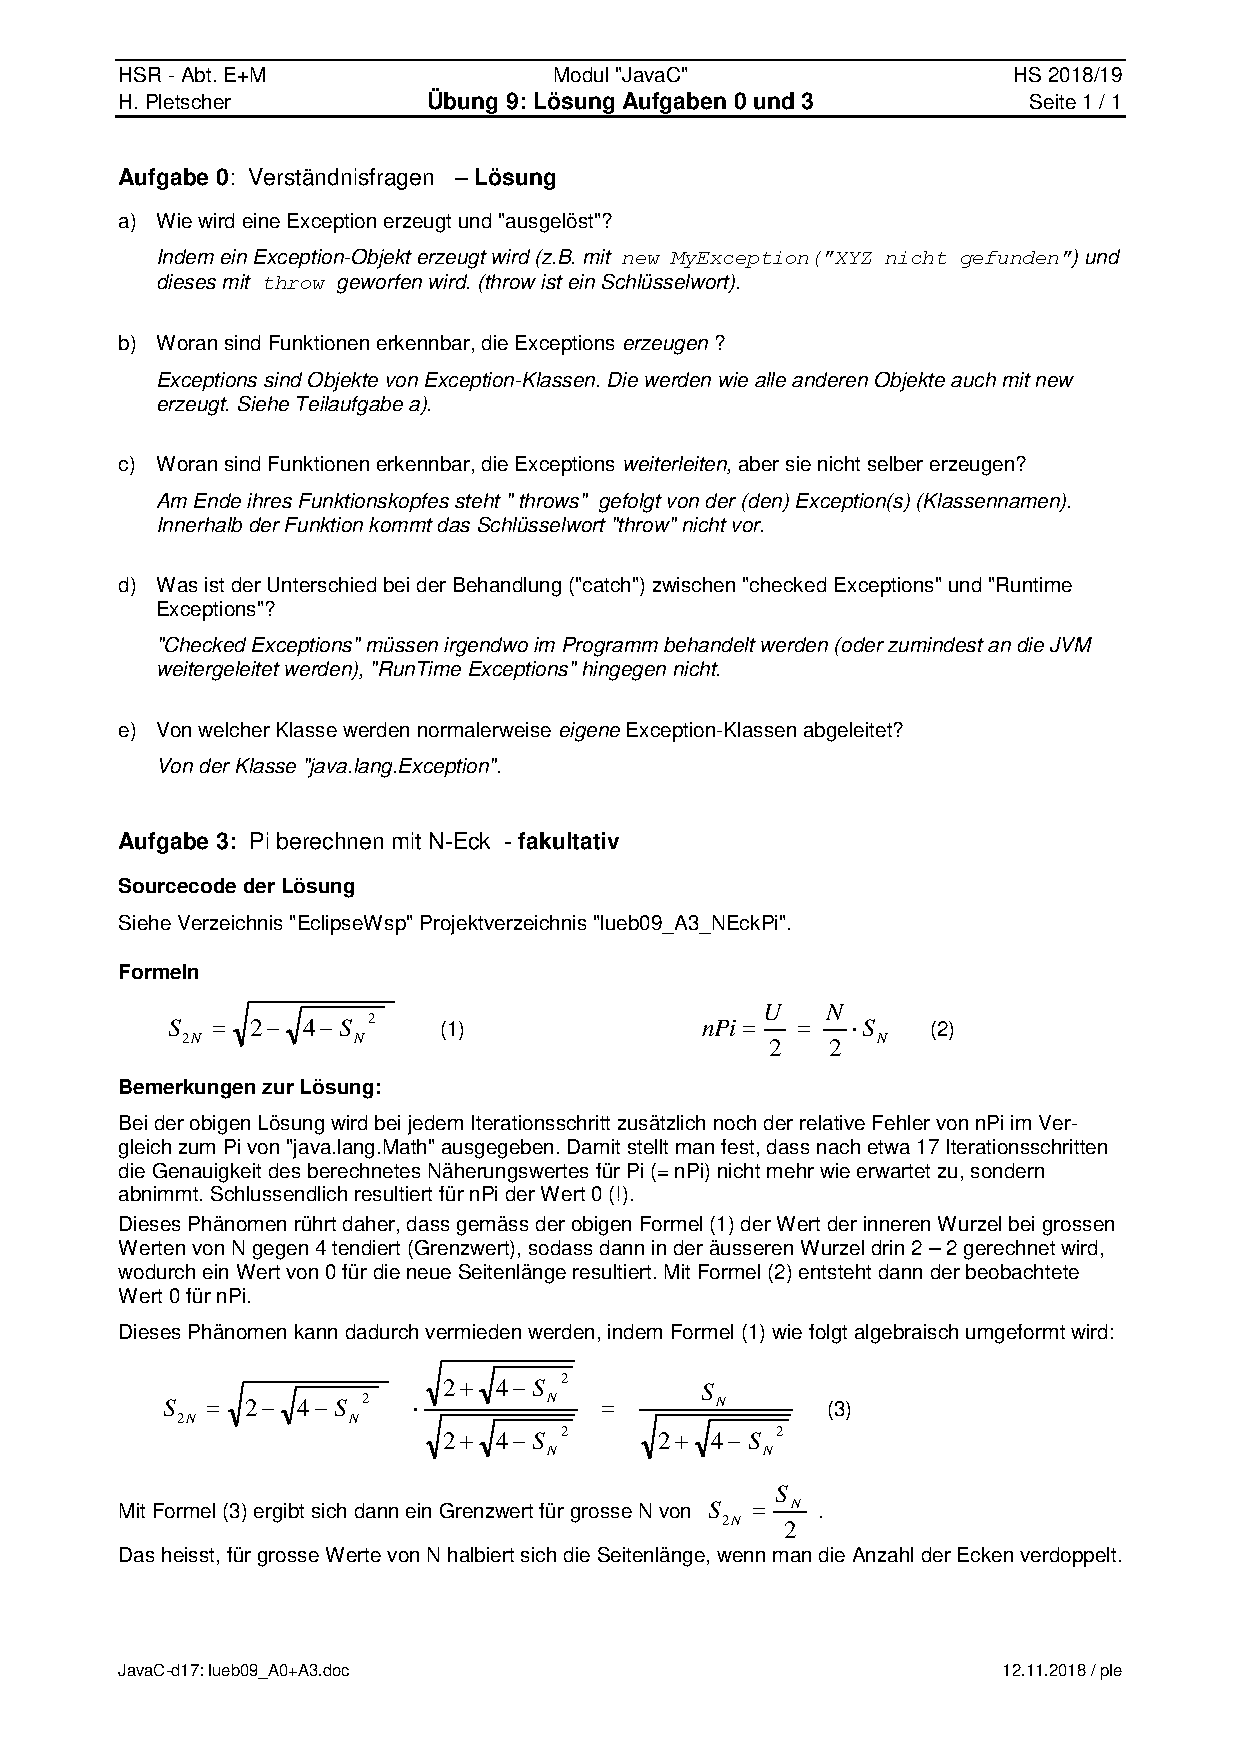
\includepdf[scale=0.9]{Loes/lueb09A0A3.pdf}
